\chapter{Sistemi RAID}
L'evoluzione logica ha permesso di avere dischi sempre pi\`u piccoli e meno costosi, pertanto \`e pi\`u facile equipaggiare un sistema con molti dischi in modo da raggiungere maggiori
prestazioni attraverso letture e scritture in parallelo e maggior affidabilit\`a tramite ridondanza. Il RAID nasce nel $1988$ come Redundant Array of Independent Disks, con l'obiettivo
di migliorare l'affidabilit\`a incrementando le prestazioni. La struttura software dei dispositivi RAID si basa su pi\`u dischi indipendenti collegati al bus e la funzionalit\`a RAID
implementata dal sistema operativo. La struttura hardware si basa su un controllore intelligente che gestisce diversi dischi collegati alla macchina. Una batteria RAID \`e un'unit\`a
a s\`e stante composta da controllore, cache e dischi autonomi collegati a una macchina, 
\section{Concetti di base}
Le strutture RAID si basano su copiatura speculare dei dati (mirroring) e sezionamento dei dati (data striping) per implementare parallelismo che garantisce aumento di prestazioni e 
affidabilit\`a. 
\subsection{Affidabilit\`a}
Un guasto a un disco comporta la perdita di dati e per migliorare l'affidabilit\`a si deve ricorrere alla ridondanza: memorizzare informazioni non strettamente necessarie ma utili per
ricostruire le informazioni perse in caso di guasto. 
\subsubsection{Copiatura speculare}
Il modo pi\`u semplice per implementare la ridondanza \`e il mirroring o shadowing in cui un disco logico corrisponde a due dischi fisici, ogni scrittura avviene su entrambi i dischi
e i dati si perdono solo se si guastano entrambi i dischi. Il tempo medio di perdita dei dati dipende dal tempo medio di guasto di ogni singolo disco e il tempo medio di riparazione. Si
noti come offra protezione solo contro i guasti indipendenti e per cause esterne entrambi i dischi potrebbero guastarsi contemporaneamente. Con mirroring la frequenza di gestione delle
letture raddoppia perch\`e si pu\`o leggere da uno qualunque dei due dischi e il tempo di trasferimento rimane inalterato. 
\subsection{Sezionamento dei dati}
Usando pi\`u dischi \`e possibile migliorare la capacit\`a di trasferimento distribuendo i dati in sezioni su pi\`u dischi (data striping). Il sezionamento pu\`o avvenire a livello di 
bit: i bit di ciascun byte vengono distribuiti su pi\`u dischi o a livello di blocco in cui i blocchi dei file sono distribuiti su pi\`u dischi. Il parallelismo tramite il bilanciamento
del carico aumenta la produttivit\`a per accessi multipli a piccole porzioni di dati e riduce il tempo di risposta relativo agli accessi a grandi quantit\`a di dati. 
\subsection{Codici per la correzione di errori}
Ad ogni byte si associa un bit di parit\`a che gli indica se gli $1$ presenti nel byte sono in numero pari (parit\`a $0$), o in numero dispari (parit\`a $1$). Identificano tutti gli 
errori su un singolo bit. Usando pi\`u bit supplementari si riescono a individuare e correggere un maggior numero di bit. 
\section{Livelli di RAID}
Il mirroring garantisce alta affidabilit\`a ma \`e costoso, mentre il data striping permette alta capacit\`a di trasferimento dati ma non migliora l'affidabilit\`a. Spesso si usano
tecniche basate sui bit di parit\`a. L'utilizzo combinato di queste tecniche \`e stato schematizzato in $6$ livelli di RAID. 
\begin{figure}[h]
	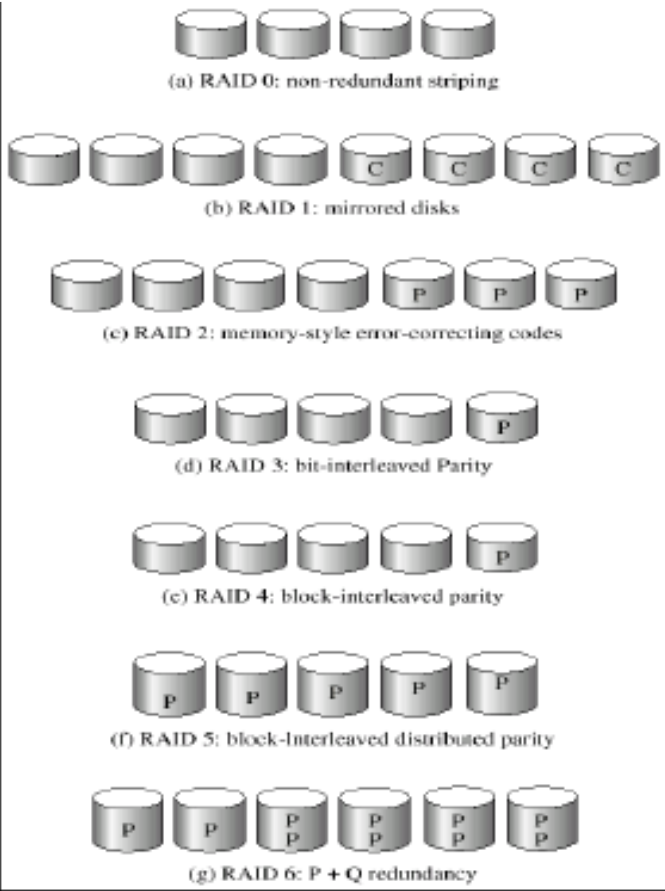
\includegraphics[width=\textwidth]{Pictures/RAID.png}
	\caption{Livelli di RAID}
\end{figure}
\subsection{Livello RAID 0}
Avviene il sezionamento a livello di blocco senza ridondanza. \`E economico e garantisce alte prestazioni grazie al parallelismo delle operazioni di lettura e scrittura. Non ha 
ridondanza e l'affidabilit\`a cala all'aumentare del numero di dischi impiegati. 
\subsection{Livello RAID 1}
Avviene mirroring senza sezionamento di blocco, aumenta l'affidabilit\`a linearmente con il numero di copie. Si aumentano le prestazioni in lettura (se il disco \`e occupato si pu\`o 
leggere dall'altro). Ha un alto costo e bassa scalabilit\`a. 
\subsection{Livello RAID 2}
Avviene il sezionamento a livello di bit e usa codici per la correzione degli errori (ECC). I bit di correzione sono memorizzati singolarmente in dischi separati diversi rispetto a 
quelli usati per i dati. Se un disco si guasta i bit rimanenti del byte dati e i bit di correzione associati vengono usati per ricostruire il dato danneggiato. Il RAID 2 richiede solo 
$3$ dischi in pi\`u per $4$ dischi dati rispetto ai $4$ richiesti dal RAID 1. Utilizza il codice Hamming che codifica $4$ bit dati in $7$ bit, aggiungendone $3$ di parit\`a. 
\subsection{Livello RAID 3}
Avviene il sezionamento a livello di byte con un disco dedicato al bit di parit\`a noto come organizzazione con bit di parit\`a. I controllori dei dischi sono in grado di rilevare se 
un settore \`e stato letto correttamente. Se un settore \`e danneggiato per ogni bit del settore \`e possibile determinare se deve valere $0$ o $1$ calcolando la parit\`a dei bit
corrispondenti dai settori degli altri dischi. Ha la stessa efficienza del RAID 2 ma usa un solo disco per i bit di parit\`a. La velocit\`a di trasferimento \`e pari a $n$ volte quella
del RAID 1. Rispetto al RAID 1 fornisce per\`o meno operazioni di I/O al secondo in quanto ogni disco \`e coinvolto da tutte le richieste e il tempo pi\`u lungo per le scritture in
quanto \`e necessario calcolare il bit di parit\`a. Pertanto il controllore RAID sar\`a capace di gestire il calcolo della parit\`a lasciando la CPU libera. 
\subsection{Livello RAID 4}
Avviene il sezionamento a livello di blocco con un disco dedicato alla parit\`a detto organizzazione con blocchi di parit\`a intercalati. \`E simile al RAID 0 con un blocco di parit\`a
in un disco separato. Ha pi\`u tolleranza ai guasti e letture pi\`u veloci grazie al parallelismo. Il disco usato per la parit\`a pu\`o esser un collo di bottiglia e le scritture sono
lente a causa del calcolo della parit\`a. 
\subsection{Livello RAID 5}
Avviene il sezionamento a livello di blocco con bit di parit\`a distribuiti tra tutti i dischi del RAID o organizzazione con blocchi intercalati a parit\`a distribuita. Un blocco di 
parit\`a non pu\`o contenere informazioni di parit\`a per blocchi che risiedono nello stesso disco. Ha gli stessi vantaggi del RAID 4 senza il collo di bottiglia del disco di parit\`a
e come esso ha scritture lente. 
\subsection{Livello RAID 6}
\`E simile al RAID 5 ma con maggiori informazioni di ridondanza per gestire guasti contemporanei su pi\`u dischi. Al posto della parit\`a usa altri codici per la correzione degli errori
come Reed-Solomon. Ha un altissima ridondanza ma \`e molto costoso e le scritture sono lente per la gestione dei codici per la correzione degli errori. 
\subsection{Livello RAID 0 + 1}
Combina 0 e 1 per fornire affidabilit\`a e alte prestazioni: si trovano due RAID 0 messi in RAID 1. Ha prestazioni migliori rispetto al RAID 5 e alta affidabilit\`a ma richiede il 
raddoppio del numero di dischi necessari alla memorizzazione dei dati e non supporta la rottura simultanea di due dischi se non appartengono allo stesso stripe. 
\subsection{Livello RAID 1 + 0}
Combina 1 e 0  per fornire affidabilit\`a e alte prestazioni: dati $n$ dischi si trovano $\frac{n}{2}$ RAID 1 in RAID 0 \`e pi\`u robusto del RAID 0 + 1 in quanto ogni disco di ogni 
stripe pu\`o guastarsi senza far perdere dati al sistema ma \`e costoso. 
